\mode<article>
Una vez se haya armado la matriz, debe resolver el sistema lineal
\begin{equation}\label{EqEcuacionSistemaLineal}
  \mathbf{A} \vec{T} = \vec{b}
\end{equation}

Utilice las subrutinas especializadas del lenguaje que haya elegido 
para implementar el método. En la figura \ref{FiguraCodeblockSolve}
se muestran las órdenes en \texttt{Matlab} y en \texttt{python}. 
Por el otro lado, en la Figura \label{FiguraResultadoTfija} se 
muestra las curvas de nivel obtenidas imponiendo temperaturas
arbitrarias en los bordes. Al mismo tiempo se muestran los ajustes
lineales de los tiempos de ejecución de las subrutinas de 
resolución del sistema lineal. 

Se usaron programas redactados en \texttt{python} y \texttt{FORTRAN}
como ejemplo de los dos tipos de lenguajes compilables y no compilables.
Por un lado, lo tiempos en \texttt{FORTRAN} son menores que en
\texttt{python}. Por otro lado, los tiempos medidos para la 
ejecución de la solución del sistema en \texttt{python} 
ajustan mal al modelo lineal, lo que se evidencia en el
mayor error en los parámetros de ajuste. Esto se debe a que
el programa \texttt{FORTRAN} se ha compilado para que la ejecución 
se implemente en un ejecutable binario que interactúa con 
la CPU `con menos intermediarios`, por decirlo de alguna 
manera. Por otro lado, el intérprete \texttt{python} 
debe pasar el programa a lenguaje de máquina en tiempo
de ejecución, lo que evidentemente insume un 
tiempo considerable.

\begin{figure}
  \includeslide[width=\textwidth]{FrameCodeblockSolve}
  \caption{Órdenes \texttt{Matlab} y \texttt{python} para 
  resolver sistemas lineales\label{FiguraCodeblockSolve} }
\end{figure}

\begin{figure}
  \includeslide[width=\textwidth]{FrameResultadoTfija}
  \caption{Resultado en el caso de bordes a temperatura fija
  \label{FiguraResultadoTfija}}
\end{figure}
%
\mode*
\begin{frame}<presentation>[label=FrameCodeblockSolve]
  \frametitle{Códigos de solución}
  
  \begin{columns}[T]
    \column{0.4\textwidth}
Resolver: \hfill    \texttt{Matlab}
    \column{0.6\textwidth}
  \begin{codeblock}
    \verbatiminput{./codexamples/solve.m}
  \end{codeblock}
  \end{columns}

  \begin{columns}[T]
    \column{0.4\textwidth}
\hfill    \texttt{ python }
    \column{0.6\textwidth}
    \begin{codeblock}
      \verbatiminput{./codexamples/solve.py}
    \end{codeblock}
  \end{columns}

  \begin{columns}[T]
    \column{0.4\textwidth}
  Graficar: \hfill \texttt{Matlab}
    \column{0.6\textwidth}
    \begin{codeblock}
      \verbatiminput{./codexamples/contourf.m}
    \end{codeblock}
  \end{columns}

  \begin{columns}[T]
    \column{0.4\textwidth}
    \hfill \texttt{python}
    \column{0.6\textwidth}
    \begin{codeblock}
      \verbatiminput{./codexamples/contourf.py}
    \end{codeblock}
  \end{columns}


\end{frame}
%
%
\begin{frame}<presentation>[label=FrameResultadoTfija]
  \frametitle{Resultado primero}
  \centering
    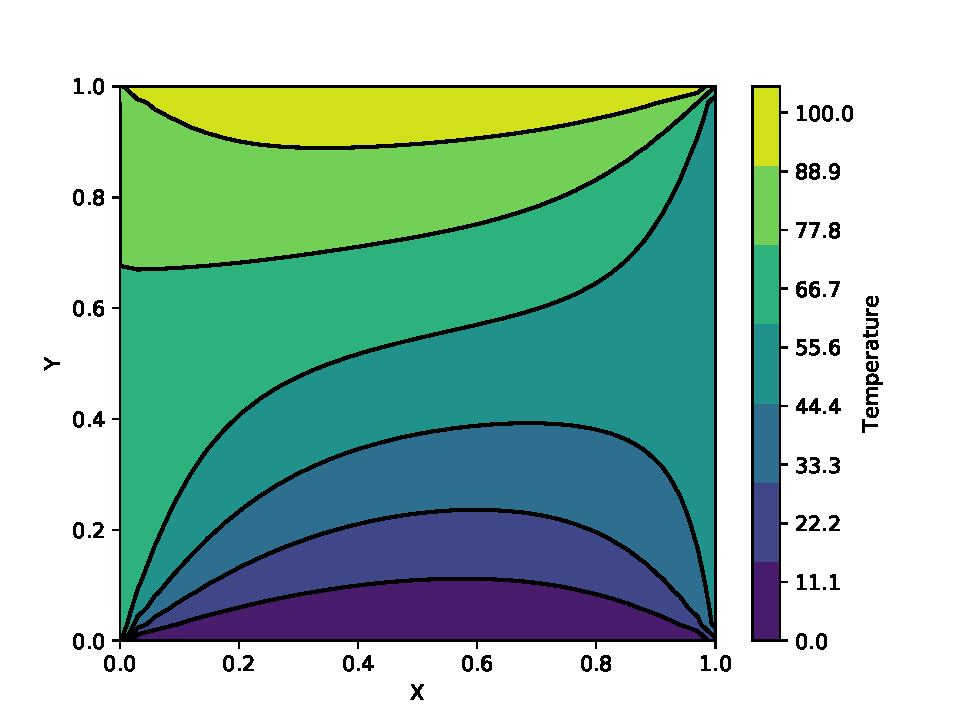
\includegraphics[width=0.4\textwidth,bb=0cm 0cm 14.5cm 12cm,clip,page=1]
    {./DATA/Temperaturas-Flujos-1.pdf}
    \hspace{1cm}
    \includegraphics[width=0.5\textwidth]{./DATA/tiempos.pdf}

\end{frame}
\mode<all>
